\documentclass{article}

\usepackage{ctex}
\usepackage{tikz}
\usetikzlibrary{cd}

\usepackage{amsthm}
\usepackage{amsmath}
\usepackage{amssymb}

\usepackage{unicode-math}


\usepackage[textwidth=18cm]{geometry} % 设置页宽=18

\usepackage{blindtext}
\usepackage{bm}
\parindent=0pt
\setlength{\parindent}{2em} 
\usepackage{indentfirst}

\usepackage{graphicx} %图片

\usepackage{xcolor}
\usepackage{titlesec}
\titleformat{\section}[block]{\color{blue}\Large\bfseries\filcenter}{}{1em}{}
\titleformat{\subsection}[hang]{\color{red}\bfseries}{}{0em}{}
%\setcounter{secnumdepth}{1} %section 序号

\newtheorem{theorem}{Theorem}[section]
\newtheorem{lemma}[theorem]{Lemma}
\newtheorem{corollary}[theorem]{Corollary}
\newtheorem{proposition}[theorem]{Proposition}
\newtheorem{example}[theorem]{Example}
\newtheorem{definition}[theorem]{Definition}
\newtheorem{remark}[theorem]{Remark}
\newtheorem{exercise}{Exercise}[section]

\newcommand*{\xfunc}[4]{{#2}\colon{#3}{#1}{#4}}
\newcommand*{\func}[3]{\xfunc{\to}{#1}{#2}{#3}}


\newcommand\Set[2]{\{\,#1\mid#2\,\}} %集合
\newcommand\SET[2]{\Set{#1}{\text{#2}}} %
\begin{document}
\title{Topology}
\author{枫聆}
\maketitle

\tableofcontents
\section{写在最前面}

拓扑对我来说是新名字,我对它几乎一无所知,虽然我嘴上总是吵吵着代数拓扑是我的终极目标\verb|(~ o ~)~zZ|,终于今天抱着巨大的勇气翻开了包志强老师的《点集拓扑和代数拓扑引论》,被文中老师幽默的行文,深深折服了,似乎拓扑也并没有想象中那么难,我想这是还不错的开始,我的第一直观感受拓扑也是给定一堆对象,在上面用一些公理弄些不一样的结构,似乎和代数一样,但是我暂时还不知道这堆结构要拿来干什么?有什么有趣的性质?

好吧,前面的路还很长,路漫漫,不过一想到前路那些绮丽的景色,多少还是有些兴奋的!虽然这路上没有一起分享喜悦的人...

2020年11月29日23:12:17

\section{Topology Space}
\subsection{Definition of Topology Space} 
预备知识

\begin{itemize}
	%\item 对于开集$U$%的理解,首先它是$X$的子集,并且对于$\forall x \in U$,存在$x$的邻域包含于$U$。包老师的书里解释为$U$是每一个$x$的邻域,我感觉在这里似乎有点强了。wiki上解释为实数轴上的开区间的一般性推广。
	\item 子集族是指$X$幂集的子集,所有子集族构成的集合则是$2^{(2^X)}$				
\end{itemize}


拓扑定义的直觉来自于微积分中连续函数的"$\varepsilon-\delta$"语言定义。

\begin{definition}
如果函数$\func{f}{\mathbb{R}}{\mathbb{R}}$满足: 任取$\varepsilon > 0$,存在$\delta > 0$使得$|x-x_0| < \delta$,对$|f(x)-f(x_0)| < \varepsilon$成立。
\end{definition}

这个定义需要$|x-x_0| < \delta$和$|f(x)-f(x_0)| < \varepsilon$这样的度量关系来定义,但是对于抽象的结构,不需要这样具体的度量关系,所以我们抽象的“邻域”来描述两点之前的具体,把所有接近$x_0$程度为$\delta$的点记做$B_{\delta}(x_0)$,这就是邻域的形式化表示,然后对于各种稀奇古怪的接近标准都可以用这个形式来表示。于是乎上面的连续定义可以稍微变一下了

\begin{proposition}
如果函数$\func{f}{\mathbb{R}}{\mathbb{R}}$满足对任意的$\varepsilon > 0$,存在$\delta > 0$有$x \in B_{\delta}(x_0)$,使得$f(x) \in B_{\varepsilon}(f(x_0))$,即$B_{\delta}(x_0) \subseteq f^{-1}(B_{\varepsilon}(f(x_0)))$
\end{proposition}

完美的略掉了度量关系,在这里$B_{\delta}(x_0)$表示$\{x \in \mathbb{R} |\ |x-x_0| < \delta \}$,最后那个包含关系是指$f(x_0)$的任何$\varepsilon$程度下的原像包含$x_0$的某个$\delta$邻域.

是否我们可以通过上面这种定义邻域的方式去把度量空间变成一般拓扑空间呢?当然是可以的,但是我们现在还没有给出邻域的一般定义。那邻域是什么?在邻域之前,应该先理解基准开邻域结构(base open neighborhood),像定义代数结构一样,基准开邻域结构是一个映射(算子)$\func{\mathcal{N}}{X}{2^(2^X)}$,把每一个点$x \in X$对应到一个子集族$\mathcal{N}(x)$上,满足下面几条公理
		\begin{itemize}
			\item $\forall x \in X,\mathcal{N}(x) \neq \emptyset,$并且$\forall U \in \mathcal{N}(x),x \in U$
			\item 若$U,V \in \mathcal{N}(x),$则存在$W \in \mathcal{N}(x)$,使得$W = U \cap V$
			\item 若$y \in U \in \mathcal{N}(x)$,则存在$V \in \mathcal{N}(y)$,使得$V \subseteq U$
		\end{itemize}
如果$U$是$x$的一个邻域,则$U$包含了某个$x$基准开邻域。用文字来叙述就是:
\begin{itemize}
	\item 每一个$x$都一定有基准开邻域,并且是其任意基准开邻域的元素
	\item $x$的任意两个基准开邻域的交是$x$的邻域
	\item 任意基准开邻域是其所含每个元素$y$的邻域
\end{itemize}

这个邻域的定义非常的奇特,那它奇特在什么地方呢?其他地方("Topology and Groupoids")关于邻域的定义是这样的:
\begin{itemize}
	\item 如果$N$是$x$的一个邻域,则$x \in N$;
	\item 如果$N$是一个包含$x$某个邻域的$X$的子集,则$N$同样是$x$的邻域;
	\item 两个$x$的邻域的交还是一个$x$的一个邻域;
	\item 如果$N$是$x$的一个邻域,且$N$包含一个$x$的邻域$M$,则$N$是$M$中所有点的邻域;
\end{itemize}

我更倾向于后面这种定义邻域的办法,不要用基准开邻域来定义,因为基准开领域其实是open neighborhood的概念,它是指它确实同时满足开和邻域的条件.这里同样可以给一个命题"如果一个子集$N$是$x$的open neighborhood当且仅当它是一个基准开邻域"。基准开邻域这个概念似乎非常old fashion,我在其他书中都没有看见过,奈何包包老师的书里有,所以这里需要好好思考一下。后面用基准开邻域的时候就想一下open neighborhood.

我们现在可以用邻域的公理来定义拓扑空间,用$\mathbf{N}$表示一个邻域拓扑,即$\mathbf{N}$表示一个所有非空的$\mathbf{N}(x)$构成的邻域族,最后$(X,\mathbf{N})$表示一个拓扑空间,这种构造方式是Hausdorff提出来的,但是一般地经常用开集的公理来定义领域。

用$(X,\uptau)$表示一个拓扑空间,其中$\uptau$表示$X$的一个子集族,并且满足下面公理:
\begin{itemize}
	\item $\emptyset \in \uptau,X \in \uptau$
	\item $\uptau$中任意两个元素的交集仍属于$\uptau$
	\item $\uptau$中任意多个元素的并集仍属于$\uptau$
\end{itemize}	
则称$\uptau$里面的元素为开集,$\uptau$表示$X$上的一个拓扑结构

开集定义的拓扑空间看起来要比邻域定义,要稍微简洁那么一点,两个定义都是等价的,你可以用邻域的推到开集。在邻域上基础上我们定义如果$U$是$X$的一个子集,且$U$是每一个$x \in U$的领域,则称$U$是一开集。基准开邻域的第三条公理告诉我们基准开邻域肯定是一个开集,然后我们给出一个命题

\begin{proposition}
一个集合是开集当且仅当它是若干个基准开领域的并集
\end{proposition}

\begin{proof}
如果当一个集合是开集时,根据开集的定义,它里面每个元素都有一个邻域,而每个邻域至少包含一个基准开邻域,因此所有基准开邻域的并构成了这个开集。反之若干个基准开领域的并,还是一个基准开领域,前面说过基准开领域是一个开集。

注意,空集也是一族基准开领域的并,只不过这个集合族是空族。
\end{proof}

这个命题证明以后,现在来看看我们用邻域定义得到的开集是否遵循开集的基本公理?很显然地,当并集是基准开领域并的情况下,是满足上诉的开集公理的。回顾前面的定义,基准开邻域在这里起了不小作用,那为什么不一开始使用基准开邻域来定义开集呢?而是使用邻域?下面引用一段包老师的话,写的真好!

基准开邻域结构(三条公理)和邻域结构(四条公理)都能刻画连续性。通常邻域结构很多,并不方便写出来,而基准邻域结构则是比较容易写出的,但它的缺点是:同一种连续性可以用不同的基准开邻域来描述。打个比方,邻域结构就是一个线性空间里面所有的向量,而基准开邻域相对于一个线性空间里面的基,所以很显然,在定义拓扑概念时,我们是希望从具有确定性的邻域结构出发去定义,等到具体计算的时候再用基准开邻域,而不是从基准开邻域结构出发去写一个表达式,用不那么确定的公式作为定义。当然邻域结构里面仍然包含很多冗余信息,因此我们最终选择另一套与之相互唯一确定的,更加简洁齐整的东西,把它称为拓扑结构(开集族)

当我们把一个拓扑空间当一个整体去研究的时候,用开集公理要比邻域的公理更加方便,领域公理似乎更强调“$x$点附近”会怎么样了?但是开集要更抽象一点,需要花些时间去理解,好吧我已经花了不少时间了!!!

\begin{example}
集合$X$上的一个平凡拓扑为$\{X,\emptyset\}$,形象一点说就是“在$X$上无论怎么着都算充分接近”,即取一个$X$作为$x$的基准开邻域,平凡拓扑是$X$上最小的拓扑结构。
\end{example}

\begin{example}
集合$X$上的一个离散拓扑为$\{X,2^{X}\}$,形象一点说就是“在$X$上只有等于$x$才算是和$x$充分接近”,离散拓扑是$X$上最大的拓扑结构。 暂时不理解为什么是等于,而不是包含,但是最大的子集族确实是$2^{X}$
\end{example}

还有两个比较重要的拓扑结构

\begin{example}
设$X$含有无穷多个元素,定义\[\tau_f = \Set{A \subseteq X}{A = \emptyset \text{ 或者 } A^c \text{ 有限}}\]则$\tau_f$是一个拓扑结构,称为$X$上的余有限拓扑(cofinite topology)
\end{example}

\begin{example}
设$X$含有不可数无穷多个元素,定义\[\tau_c = \Set{A \subseteq X}{A = \emptyset \text{ 或者 } A^c \text{ 可数}}\]则$\tau_c$也是一个拓扑结构,称为$X$上的余可数拓扑(cocountable topology)
\end{example}

这里还是有必要讲一下度量是什么东西,因为后面有很多东西都是,欧式度量诱导出来的度量拓扑.一个度量就是测量空间中两个点之间距离的一个公式. 当然,为了确保这个公式真的能起到类似距离的作用,它还需要满足一些基本的公理.

\begin{definition}
$X$上的一个度量(metric)是一个映射\[\func{d}{X \times X}{\mathbb{R}}\]满足
\begin{enumerate}
	\item \textbf{正定性}(positive definite) $\forall x,y \in X,d(x,y) \geq$,并且$d(x,y)=0$当且仅当$x=y$;
	\item \textbf{对称性}(symmetry) $\forall x,y \in X,d(x,y)=d(y,x)$;
	\item \textbf{三角不等式}(triangle inequality) \[\forall x,y,z \in X,d(x,z) \leq d(x,y)+d(y,z)\].
\end{enumerate}
$X$和$d$合起来叫一个\textbf{度量空间}(metric space),记做$(X,d)$.
\end{definition}

然后呢,在度量空间中可以定义一个自然的基准开邻域结构如下: 考虑那些$B_{\varepsilon}(x)=\Set{y \in X}{d(x,y) < \varepsilon}$.我们称之为$x$的$\varepsilon$-球心邻域($\varepsilon$-ball).取$\mathcal{N}_d(x)=\Set{B_{\varepsilon}(x)}{\varepsilon \> 0}$.

\begin{proposition}
其中$\mathcal{N}_d$确实是$X$上的一个基准开邻域结构.由$\mathcal{N}_d$生成的拓扑$\tau_d$称为度量空间$(X,d)$上的度量拓扑(metric topology).
\end{proposition}

\begin{proof}
需要证明$N_d$满足基准开邻域结构的三条公理:
\begin{enumerate}
	\item $x \in B_\varepsilon(x)$,显然地;
	\item $B_{min(\varepsilon,\delta)}(x)=B_{\varepsilon}(x) \cap B_{\delta}$
	\item 任取$y \in B_{\varepsilon}(x)$,要给它也找一个基准开邻域$B_{\delta}(y)$包含于$B_{\varepsilon}(x)$,那么$B_{\delta}(y)$里面的点也应该是属于$B_{\varepsilon}(x)$,我们不妨再设一点$z \in B_{\delta}(y)$,即$d(y,z) < \delta$,确定合适的$\delta$要求$d(x,z) < \varepsilon$,由三角不等式我们有下面不等式 \[\left\{
		\begin{array}{l}
			d(x,z)\leq d(x,y) + d(y,z) \\ 
			d(y,z) < \delta  \\ 
			d(x,z) < \varepsilon 
		\end{array}
	\right.\]由(1)和(2)可得$d(x,z) < \delta + d(x,y)$,所以我们只需要取$\delta = \varepsilon - d(x,y)$即可.
\end{enumerate}
\end{proof}

\begin{definition}
设$\tau_\varepsilon$是$\mathbb{R}^n$上欧式度量所决定的拓扑,则拓扑空间$(\mathbb{R}^n,\tau_\varepsilon)$为一个$n$维\textbf{欧式空间}(Euclidean space),记为$\mathbb{E}^n$.
\end{definition}

\newpage
%https://math.stackexchange.com/questions/157735/definition-of-neighborhood-and-open-set-in-topology
\subsection{Properties of Topology Space}

一般的基本定义都会从开集出发,如何从开集出发去定义邻域呢?

\begin{proposition}
一个子集$A$是$x$的邻域当且仅当存在开集$U$,使得$x \in U \subseteq A$.
\end{proposition}

\begin{proof}
从左边证右边,很显然,因为当$A$是$x$的邻域时,可以找到一个$x$的一个基准开邻域,这个基准开邻域也是一个开集,这个还可以用interior来证明,interior就是一个开集。\\
从右边证左边,稍微有点繁琐但是呢,也好证,先给定邻域子集族\[\mathcal{N}(x)=\Set{A}{A \supseteq U, \text{U是一个开集}}\],然后从邻域的4条公理出发:
\begin{enumerate}
	\item $x \in U \subseteq A$,这个很显然.
	\item $A' \subseteq A \subseteq U$,所以$A' \in \mathcal{N}(x)$.
	\item 给定一个$A' \subseteq U'$,其中$U'$也是一个开集,然后呢我再设${U'}^c=A' \smallsetminus U'$,相同地$U^c= A \smallsetminus U$,那么$A' \cap A =({U'}^c \cup U') \cap (U^c \cup U)= (U'^c \cap U^c) \cup (U'^c \cap U) \cup (U' \cap U^c ) \cup (U' \cap U)$.其中$U' \cap U$是一个开集,所以$A' \cap A \in \mathcal{N}(x) $.
	\item 任意的$x \in A$,总能找到一个$A' = \{x\} \cup U \subseteq A$,且$A' \in   \mathcal{N}(x)$.
\end{enumerate}

终于完整证完了,其他书上的证明都很简单,给我一种循环论证的感觉。
\end{proof}

%\begin{enumerate}
%	\item $x \in U \subseteq A$
%	\item $x \in $
%\end{enumerate}
%\end{proof}

%\begin{proof}
%只需要证明这样定义出来的邻域是满足上面那4条公理的就行,除了第三条其他的都比较显然,怎么证明第三条呢?$U$是一个开集,$U$自己包含自己,任意$x \in U$,根据开集给出的邻域定义,$U$是$x$的邻域,这样第三条我们也证明了,哈哈,包老师在这里的证明似乎循环论证了lol
%\end{proof}


\begin{definition}
如果$A$是$x$的邻域,则称$x$为$A$的\textbf{内点}(interior point).全体内点构成的集合称为\textbf{内部}(interior),记做$A^{\circ}$
\end{definition}

内点和内部的概念,需要建立在具体的拓扑结构上,取不同的拓扑结构会得到完全不同的结论。

\begin{center}
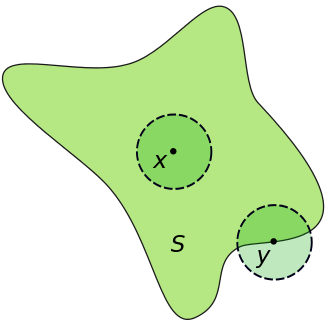
\includegraphics[width=5cm, height=4cm]{images/Interior_illustration.png}
\end{center}

interior有一个性质很重要就是interior是其内部所有点的邻域。

\begin{proof}
假设$M$是$x$的邻域,且$M \subseteq A$,那么$M$里面的所有点都有一个邻域含于$M$,也含于$A$,所以$A$是$M$所有点的邻域,自然地$M \subseteq A^{\circ}$,所以$A^{\circ}$是$x$的邻域,这里的$x$是任意地。
\end{proof}


\begin{proposition}
集合的内部具有以下基本性质:
\begin{itemize}
	\item $A^{\circ}=A$当且仅当$A$是开集;
	\item $A^{\circ}$是$A$包含的所有开集的并集,也是$A$中最大的开集;
	\item 若$A \subseteq B$,则$A^{\circ} \subseteq B^{\circ}$;
	\item $(A_1 \cap \ldots \cap A_n)^{\circ}=A_1^{\circ} \cap \ldots \cap A_n^{\circ}$;
	\item ${\left(\bigcup\limits_{i \in n} A_i\right)}^{\circ} \supseteq \bigcup\limits_{i \in n} A_i^{\circ}$
\end{itemize}
\end{proposition}
\begin{proof}
\begin{enumerate}
	\item 这个性质根据开集的定义很显然。
	\item 如果$A$的子集是一个开集,这个子集很显然也是属于$A^{\circ}$,所以$A$里面的所有开集含于$A^{\circ}$,如何证明$A^{\circ}$是一个开集呢?任取$A^{\circ}$中一点$x$,$A$是x的邻域,那么一定存在一个包含$x$的基准开邻域,我们最大基准开邻域是一个并集,根据基准开邻域的定义,这个基准邻域肯定也是属于$A^{\circ}$,所以$A^{\circ}$是其每个点$x$的邻域,所以$A^{\circ}$是一个开集,同时也证明了它是所有这样点$x$的基准开邻域的并。再来证明它是$A$内最大的开集,假设如果它不是$A$内最大的开集,那么存在$A^{'}$包含$A^{\circ}$,但是呢$A'$是其所有点的邻域(根据开集定义),所有$A'$属于$A^{\circ}$,这样产生了矛盾,所以$A^{\circ}$是最大的开集。
	\item 根据邻域的最后一条公理,邻域的超集还是邻域,所以B是$A^{\circ}$中所有点的邻域,所以很自然的$A^{\circ} \subseteq B^{\circ}$
	\item 等式的左边表示,所有集合的交的内部,等式的右边表示,所有集合的内部的交,这里为什么等价呢?这个关系用图来说是非常明显的,怎么用文字呢?应该用数学归纳法来证明,我先证明对两个集合是成立的,首先利用第2个性质,${(A_1 \cap A_2)}^{\circ}=U_1 \cup \ldots \cup U_n $,其中$U_1,\ldots,U_n \in A_1 \cap A_2$,很显然它们也属于$A_1^{\circ}$和$A_2^{\circ}$,即${(A_1 \cap A_2)}^{\circ} \subseteq A_1^{\circ} \cap A_2^{\circ}$,反过来$A_1^{\circ} \cap A_2^{\circ}$是一个开集,并且属于$(A_1 \cap A_2)$,所以$A_1^{\circ} \cap A_2^{\circ} \subseteq {(A_1 \cap A_2)}^{\circ}$,两边一夹所以,${(A_1 \cap A_2)}^{\circ} = A_1^{\circ} \cap A_2^{\circ}$,再用一下数学归纳法,即可。
	\item 这个也需要数学归纳法来证明,这里只证明两个集合的情况下,$A_1^{\circ} \cup A_2^{\circ} \subseteq {(A_1 \cup A_2)}^{\circ}$这还是显然的,用第三条性质就可以知道。但是反过来不一样成立,$A_1$和$A_2$的"公共边界"上的点,完全有可能变成$A_1 \cup A_2$内部的点。
	\begin{center}
		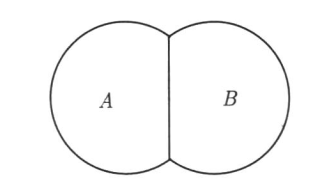
\includegraphics[width=4cm, height=2cm]{images/A_B_same_border.png}
	\end{center}	
\end{enumerate}
\end{proof}

\begin{definition}
如果在拓扑空间$(X,\tau)$中,子集$A$的余集$A^{c}$是开集,则称$A$为\textbf{闭集}(closed set)
\end{definition}

其中余集$A^{c}= X \smallsetminus A$,在平凡拓扑中,闭集就是$\emptyset$和$X$;在离散拓扑中,任何子集都是闭集;闭集和开集互为余集,也可以从闭集出发定义拓扑结构:

\begin{definition}
$X$的子集族$\sigma$是某个拓扑结构下全体闭集构成的集合当且仅当它满足下述三条公理:
\begin{itemize}
	\item $X \in \sigma$,$\emptyset \in \sigma$;
	\item $\sigma$中任意多个元素的交集仍属于$\sigma$;
	\item $\sigma$中任意两个元素的并集仍属于$\sigma$;
\end{itemize}
\end{definition}

我们尝试来推一下开集公理,第一个公理很显然,主要看第二个和第三个,开集和闭集互为余集,如果$A$和$B$为闭集,则$A^c$和$B^c$为开集,根据De Morgan定律\[A^c \cup B^c = (A \cap B)^c , A^c \cap B^c = (A \cup B)^c\],根据闭集公理,上面两个等式结果都是开集。

\begin{definition}
如果$x$每个邻域中都含有$A \smallsetminus \{x\}$中的点,则称$x$为$A$的聚点或者极限点(limit point 或 cluster point 或 point of accumulation),全体聚点构成的集合$A'$称之为$A$的导集(derived set),$\overline{A}=A \cup A'$称为$A$的闭包(closure).换言之,$x \in \overline{A}$当且仅当$x$的每个邻域中都含有$A$中的点。
\end{definition}

突然多了很多定义,让人触不及防,因为一开始不知道它们的深刻含义。这个定义感觉很模糊,因为没有给$A$到底是什么东西,$x$和$A$关系是什么?

假设$A$是任意给定一个$X$的子集,那么$x$也是任意取的,所以两者并没有直接关系,而是靠上面刻画的几个关系,首先把用聚点的定义,把$x$和$A$联系起来,然后把这样的$x$都找出来,于是就有全体聚点这个概念,再给它一个定义为导集,把导集和$A$本身并起来,再给一个定义就是闭包。

上面重新解读了一下定义,那么再研究一下这个闭包有什么性质?闭包$\overline{A}$中任意一点$x$,如果$x \in A'$,则$x$的每个邻域都含有$A$中的点。如果$x \in A$,怎么推出和前面一样的结论呢?注意这样好像只需要含有就行,不需要全含,所以$x$本身在$A$里面这个条件是天然成立的。

\begin{proposition}
设$A$是$X$的一个子集,则$(A^{c})^{\circ}=(\overline{A})^c$.
\end{proposition}

\begin{proof}
这个命题在说明内部和闭包的关系,从右边出发好像简单一点,$A$的闭包的余集,是指那些点$x$的邻域都不包括$A$中的点。换句话说就是指点$x$有一个邻域都只包含$A^c$的点,则这个邻域是含于$A^c$,根据内点的定义,点$x$是$A^c$的内点,所有这样的点,就是$(A^c)^{\circ}$.总结一下就是$A$的闭包和$A^c$的开集互为余集。	
\end{proof}

于是,所有关于内部的性质都可以用De Morgan定律翻译成闭包的性质。

\begin{itemize}
	\item $\overline{A} = A$,当且仅当$A$是闭集。
	\item $\overline{A}$是包含$A$的所有闭集的交集,也是包含$A$的最小闭集。
	\item 若$A \subseteq B$,则$\overline{A} \subseteq \overline{B}$
	\item $(A_1 \cup \ldots \cup A_n)^{\circ}=A_1^{\circ} \cup \ldots \cup A_n^{\circ}$;
	\item ${\left(\bigcap\limits_{i \in n} A_i\right)}^{\circ} \subseteq \bigcap\limits_{i \in n} \overline{A_i}$
\end{itemize}

\begin{proof}
我尝试用$(A^{c})^{\circ}=(\overline{A})^c$,来简单证明一下第一条,若$\overline{A}=A$,则$(\overline{A})^c = A^c=(A^{c})^{\circ}$,后面这个根据内部的性质则$A^c$是开集,所以$A$为闭集(开集和闭集互为余集)。
\end{proof}


\begin{definition}
如果$\overline{A}=X$,则称$A$在$X$中稠密(dense)。如果$X$有只含有可数多个元素的稠密子集,则称$X$可分(separable).
\end{definition}

这个定义有点抽象,第一个话是指,定义$X$某个子集$A$,如果对$X$中任意的点$x$,要么属于$A$或者是$A$的一个聚点,则称$A$在$X$中是稠密的。非正式说法是,对于$X$中任意的点$x$,要么属于$A$或者“任意接近”$A$中的某个点。

\begin{example}
有理数集是实数集一个稠密集,因为每一个实数,可能是一个有理数或者存在一个任意接近它的有理数(丢番图近似)。
\end{example}

\begin{example}
用$\tau_f$表示$\mathbb{R}$上的余有限拓扑,则$(\mathbb{R},\tau_f)$可分,$\mathbb{N}$就是它的一个可数稠密子集。但是为什么呢?首先$\mathbb{N}$可数就不用说了,那么为什么$\mathbb{N}$是稠密的呢?根据闭包的性质,$\overline{\mathbb{N}}$等于所有包含$\mathbb{N}$闭集的交集。再根据余有限拓扑的定义,其闭集是有限的,但是不存在包含$\mathbb{N}$的有限闭集,那包含$\mathbb{N}$只有$\mathbb{R}$了,所以$\overline{\mathbb{N}}=\mathbb{R}$.
\end{example}

\begin{example}
用$\tau_c$表示$\mathbb{R}$上的余可数拓扑,则$(\mathbb{R},\tau_c)$不可分。任意的$\mathbb{R}$的可数子集$U$,在余可数拓扑上都是闭集,而闭集的闭包是自己,$U \neq \mathbb{R}$,所以不存在这样的可数子集。
\end{example}

\newpage
\subsection{Potency of Set and countable set}

对于一个空间来说,比拓扑性质和概念更基本的是它作为集合的那些性质和概念。

\begin{definition}
设$A$,$B$是两个集合。如果存在双射$\func{f}{A}{B}$,则称$A$和$B$的基数(cardinality)或者势(potency)相等,记做$\|A\|=\|B\|$.
\end{definition}

\begin{lemma}
如果$A$,$B$是有限集,则$\|A\|=\|B\|$当且仅当它们所含的元素相等.
\end{lemma}

\begin{lemma}
如果$A$是无限集,则它必有一个可数无限集
\end{lemma}

\begin{proof}
按顺序每次取一个就行。
\end{proof}

\begin{proposition}
集合$A$无限当且仅当它与一个真子集基数相等.
\end{proposition}

%https://proofwiki.org/wiki/Infinite_Set_is_Equivalent_to_Proper_Subset
\begin{proof}
这个命题值得证明一下,从前面第一个lemma我们知道,如果$A$和真子集基数相等,那它肯定不是有限集。反过来$A$如果不是有限集,则它是无限集,第二lemma可知,我们可以构造一个可数无限集$S=\{a_1,a_2,\ldots\}$,然后对它再分一个类:\[S_1 = \{a_1, a_3, a_5, \ldots\}, S_2 = \{a_2, a_4, a_6, \ldots\}\]再建立一个$S$和$S_1$之间的双射$a_n \leftrightarrow a_{2n-1}$,然后再把这个双射扩展到$S \cup (A \smallsetminus S) = T$ 和 $S_1 \cup (A \smallsetminus S) = A \smallsetminus S_2$,都并上了$A \smallsetminus S$,所以把$a \in A \smallsetminus S$映到它自己就行,还是维持$S$和$S_1$的映射。所以现在建立了一个$A$与$A \smallsetminus S_1$的双射。这个证明看起来就没有那么违反直觉,不错不错。
\end{proof}

\begin{theorem}
Cantor-Schroder-Bernstein,if $|A|\leq|B|$ and $|B|\leq |A|$,then $|A|=|B|$.
\end{theorem}

\begin{proof}
定义两个单射$\func{f}{A}{B}$和$\func{g}{A}{B}$.想象下面的序列:\[\cdots \rightarrow  f^{-1}(g^{-1}(a)) \rightarrow g^{-1}(a) \rightarrow   a  \rightarrow  f(a) \rightarrow  g(f(a)) \rightarrow \cdots\],其中$a \in A$,从$a$点往左好理解,就是重复使用$f$,$g$,那从$a$点往右呢?也很好理解,就是重复使用$f^{-1}$和$g^{-1}$,但是呢它可能到某个位置就停了,因为有可能某个地方它们没有定义了,因为我们只保证了$f$和$g$是一个单射。先理解这个性质,我们再来想办法用$f$和$g$构造一个$\func{h}{A}{B}$的双射.

按照上面的理解,这个序列有三种情况:
\begin{itemize}
	\item 从a点出发转一圈,有转回来了。其实就是指这条路径上的$f^{-1}$和$g^{-1}$都有定义。
	\item 想象一直往左边看,如果某个点$f^{-1}$没有定义,那么其实就在某个$x \in B$位置停下了。
	\item 想象一直往左边看,如果某个点$g^{-1}$没有定义,那么其实就是就在某个$x \in A$位置停下了。	
\end{itemize}

先看后面两种情况,如果在B点停下了,那么我们就让$h(x)$在这点$h^{-1}(x)=g(x)$,即$h(x)=g^{-1}(x)$,现在我们确定了一个点的对应关系,为什么可以这样取呢?因为$g(x)$是单射,确定这点对应的两点之前关系是唯一的,也就是$g(x)$引出的箭头是唯一的(因为$f^(-1)$在这点没有定义了,我们考虑这点的$g^{-1}$.)。对应的如果在A点停下了,我们就让$h(x)=f(x)$.那么是一个循环序列我们怎么吗?那么对应这个循环序列里面连着的两点,统一用$g^(-1)$或者$f$来表示对应关系,即可。下图,做一个形象记忆,采自wiki。

\begin{center}
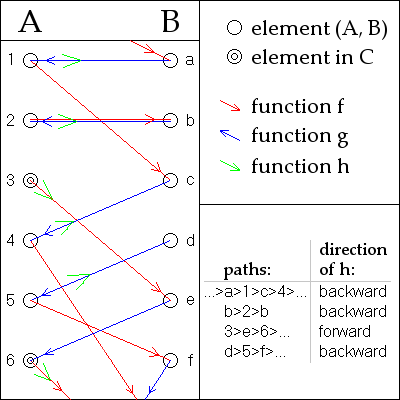
\includegraphics[width=10cm, height=8cm]{images/Cantor-Bernstein.png}
\end{center}

König's definition of a bijection h:A → B from given example injections f:A → B and g:B → A. An element in A and B is denoted by a number and a letter, respectively. The sequence 3 → e → 6 → ... is an A-stopper, leading to the definitions h(3) = f(3) = e, h(6) = f(6), .... The sequence d → 5 → f → ... is a B-stopper, leading to h(5) = g−1(5) = d, .... The sequence ... → a → 1 → c → 4 → ... is doubly infinite, leading to h(1) = g−1(1) = a, h(4) = g−1(4) = c, .... The sequence b → 2 → b is cyclic, leading to h(2) = g−1(2) = b.

\end{proof}


\begin{definition}
若$\|A\| \leqslant \|\mathbb{N}\|$,则称$\|A\|$可数。 
\end{definition}

显然可数集的子集一定也是可数集,并且可数无限集一定和$\mathbb{N}$基数相等。

著名的连续统假设,$\|\mathbb{R}\|$是不是就是紧挨着$\|\mathbb{N}\|=\mathcal{N}_0$的最小基数呢?
\newpage
\subsection{Continuous map and homeomorphism}

\begin{definition}
设$X$,$Y$是两个拓扑空间. 如果映射$\func{f}{X}{Y}$满足: 任取$f(x_0)$的邻域$V$,$f^{-1}(V)$都是$x_0$的邻域,则称$f$在$x_0$处\textbf{连续}(continuous). 在定义域上处处都连续的映射称为\textbf{连续映射}(continuous map).
\end{definition}

这个定义要注意的是,连续的条件是“邻域的原像是邻域”,而不是“邻域的像是邻域”,这个地方要想一想,参考函数连续,出发是从$f(a)$的接近程度来找到合适的$x$接近$a$.

\begin{example}
不论$X$,$Y$是什么拓扑空间,取定$b \in Y$,\textbf{常值映射}(constant map)\[\func{e_b}{X}{Y},\ x \mapsto b\]是连续映射,因为$b$的任意邻域的原像都是全空间$X$.
\end{example}

这个逆映射的定义是啥?奇奇怪怪的,直接找原像不就完了吗?:)

\begin{example}
拓扑空间$X$上的\textbf{恒同映射}(identity map)\[\func{id_{X}}{X}{X},\ x\mapsto x\]是连续映射,因为每个邻域的原像都是它本身.注意这里的定义域和值域都是相同的拓扑结构。
\end{example}

\begin{proposition}
对$X$和$Y$分别取定能生成对应结构的基准开邻域结构,则$f$在$x_0$处处连续的充分必要条件是: $f(x_0)$的任何基准开领域$U$的原像$f^{-1}(U)$包含一个$x_0$的基准开邻域.
\end{proposition}

\begin{proof}
基准开邻域也是一个邻域,必要性比较显然,主要看充分性如何证明,$f(x_0)$的任意邻域$U$都有一个基准开邻域$U_0$,即$U \supseteq U_0$,那么$f^{-1}(U) \supseteq f^{-1}(U_0)$,所以$f^{-1}(U)$同样包含一个基准开邻域,即$f$在$x_0$处连续。
\end{proof}

\begin{example}
设$X$,$Y$都是度量拓扑空间,则上述命题说明$\func{f}{X}{Y}$在$x_0 \in X$连续当且仅当$f(x_0)$的任意球形邻域的原像,包含一个$x_0$的球形邻域,这个条件可以进一步改写为:\[\forall \vartheta ,\exists \delta,\text{ 使得 } d_X(x,x_0) < \delta \text{ 蕴含 }d_Y((f(x),f(x_0)) < \vartheta\]
\end{example}

\begin{proposition}
若$\func{f}{X}{Y}$在$x$点连续,$\func{g}{Y}{Z}$在$f(x)$点连续,则$\func{g \circ f}{X}{Z}$在$x$点连续。
\end{proposition}

\begin{proof}
这个命题说明连续的复合还是连续,按照定义来证明,任取$g(f(x))$的邻域$U$,则$g^{-1}(U)$是$f(x)$的邻域,接着$f^{-1}(g^{-1}(U))$是$x$的邻域,因为$(g \circ f)^{-1}(U)=f^{-1}(g^{-1}(U))$,证毕。
\end{proof}

前面用了太多邻域的概念,不妨用本原开集来定义一下连续的概念

\begin{theorem}
考虑一个映射$\func{f}{X}{Y}$,下述两个条件都是$f$为连续映射的充分必要条件:
\begin{enumerate}
	\item $Y$中任意开集关于$f$的完全原像都是$X$中的开集.
	\item $Y$中任意闭集关于$f$的完全原像都是$X$中的闭集.
\end{enumerate}
\end{theorem}

\begin{proof}
从邻域定义的开集出发,先证(1)必要性: 任取$Y$中的开集$U$,对$\forall f(x) \in U$,有$f^{-1}(U)$是$x$的邻域($U$是$f(x)$的邻域,再根据$f$连续),由于$x$是任意的,所以$f^{-1}(U)$是一个开集(根据开集的定义).

再证(1)的充分性: 任取$x \in X$以及$f(x)$的邻域$V$,则存在开集$U$使得$f(x) \subseteq U \subseteq V$,根据命题$f^{-1}(U)$也是一个开集,而$x \in f^{-1}(U) \subseteq f^{-1}(V)$,所以$f^{-1}(V)$是一个邻域.	

(2)的充分必要性,由一个有趣的事实决定: \[f^{-1}(U)^c  = f^{-1}(U^c)\],如果$U^c$是一个开集,那么$f^{-1}(U)$就是一个闭集,同样$U$也是一个闭集。
\end{proof}

\begin{definition}
如果$\func{f}{X}{Y}$是一个双射,并且$f$和$f^{-1}$都连续,则称$f$为\textbf{同胚}(homeomorphism),并且称$X$与$Y$\textbf{同胚}(homeomorphic)或者\textbf{拓扑等价},记为$X \cong Y$.
\end{definition}

同胚的空间具有本质上一样的连续性.仔细想想这个定义可能在刚开始,会有一并且对于每个指标$\lambda in \Lambda$,取定一个拓扑空间$(Y_\lambda,\tau_\lambda)$以及一个映射$\func{\lambda}{X}{Y_\lambda}$些疑惑,在$\mathbb{R}$上,如果一个$f$是双射,且$f$连续,那为什么还要保证$f^{-1}$连续呢?直觉上前两个条件似乎可以直接保证$f$的逆映射是连续的。

注意这里是连续是拓扑结构上的概念,两个集合之前的一一对应,再确定分别确定两个集合上的拓扑结构之前,啥也保证不了。只有再两个对应的拓扑结构确定以后,我们再来讨论这里的连续到底是什么.举个很显然的例子,说明$f$是双射,$f$是连续的,但是$f$的逆并不连续。

\begin{example}
设$\func{f}{X}{Y}$是一个双射,然后我取$X$上的拓扑结构为离散拓扑,$Y$上的拓扑结构为平凡拓扑。显然在$f$上是连续的,因为不管$f(x)$取什么,其原像对应的子集都是开集,但是反过来$f^{-1}$,就可能不是连续了,因为$Y$上拓扑就两个元素,我大可以找很多$X$上的邻域,对应到$Y$上,并不在这样拓扑里面.
\end{example}

这样看来同胚,其实就是我们在给定一一对应的集合映射上,需要再去关注拓扑结构之间的关系,也就是所谓的连续.

\begin{theorem}
同胚是拓扑空间之间的等价关系.我们称一个关系$\cong$是\textbf{等价关系}(equivalence relation),如果它满足:并且对于每个指标$\lambda in \Lambda$,取定一个拓扑空间$(Y_\lambda,\tau_\lambda)$以及一个映射$\func{\lambda}{X}{Y_\lambda}$
\begin{enumerate}
	\item 自反性(reflexivity) $X \cong X$
	\item 对称性(symmetry) 如果$X \cong Y$,则$Y \cong X$ 
	\item 传递性(transitivity) 如果$X \cong Y$,则$Y \cong Z$,则$X \cong Z$
\end{enumerate}
\end{theorem}

\begin{proof}
\begin{enumerate}
	\item 恒同映射$\func{id_X}{X}{X}$.
	\item 同胚的定义.
	\item 前面的提到连续的复合映射,就可以用到这里.
\end{enumerate}
\end{proof}

注意前面的$X$,$Y$,$Z$都表示拓扑空间,就是指对应的各自已经先确定好了拓扑,在这里不要造成歧义。

\begin{definition}
在同胚下保持不变的性质叫拓扑性质(topological property),在同胚下保持不变的概念称为\textbf{拓扑概念}(topological concept),在同胚下保持不变的量称为\textbf{拓扑不变量}(topological invariant).
\end{definition}

对各种类型的拓扑空间进行同胚分类,是拓扑学最基本的研究课题之一。证明两个空间同胚,只要想办法把同胚映射构造出来就行了。而要区分两个空间不同胚,只需要证明一个空间满足某种性质,而另一空间不满足该性质,或者证明对两个空间算某种拓扑不变量的时候,计算结果不同。


\newpage
\subsection{Product topology}
这章主要讲如何构造一个拓扑结构?这里有一种非常有趣的定义拓扑结构的方法.设有一个映射$\func{f}{X}{Y}$,集合$X$上尚未确定具体的拓扑结构,而集合$Y$上有个拓扑结构$\mu$,则可以利用$f$把这个拓扑"向左转移"到$X$上,即取$\tau$为$X$上使得$\func{f}{(X,\tau)}{(Y,u)}$连续的最小拓扑(最小的概念是指最小的$X$的子集族).

这个方法可以推广到一族映射$\func{f_\lambda}{X}{Y_\lambda}$上,相应地得到的拓扑就是$X$上所谓的"弱拓扑".类似地,也有一套利用映射"向右转移"拓扑结构的方法,相应地得到的拓扑就是$Y$上的"强拓扑".弱拓扑和强拓扑作用,都是利用映射把一个空间上的拓扑结构以最能充分利用该映射的方式转移到另一个空间上去.

弱拓扑和强拓扑的观点主要是让我们理解这些拓扑"为什么这样定义".


\begin{definition}
考虑一个集合$X$.设$\Lambda$是一个指标集,并且对于每个指标$\lambda \in \Lambda$,取定一个拓扑空间$(Y_\lambda,\tau_\lambda)$以及一个映射$\func{f_\lambda}{X}{Y_\lambda}$.则$X$上满足条件每个$\func{\lambda}{X}{Y_\lambda}$都连续的最小拓扑$\tau$称为由这些$f_\lambda$决定的\textbf{弱拓扑}(weak topology).
\end{definition}

注意前面已经提到过的最小的含义,如果更形式化的理解是:如果有其他拓扑$\mu$也满足上述条件,则$\tau \subseteq \mu$.

那么如何构造这个弱拓扑呢?很显然有一个拓扑是天然满足的上述条件的,那就是离散拓扑.但是我们寻找是符合这样条件的一个最小的拓扑。上述条件也可以理解为要求每个$Y_\lambda$中开集的原像都是开集,所以$\tau$是包含这些原像的,但是只包含这些原像是不够的,因为我们并不能保证这些原像的交或者并是满足开集公理的,解决办法是把这些有限原像的交和任意的原像的并也取做开集。

\begin{proposition}
设$\Lambda$是一个指标集,并且对于每个指标$\lambda \in \Lambda$,取定一个拓扑空间$(Y_\lambda,\tau_\lambda)$以及一个映射$\func{f_\lambda}{X}{Y_\lambda}$.取 \[\mathcal{U}(x)=\Set{f_{\lambda}^{-1}(U_\lambda)}{\lambda \in \Lambda,f_\lambda(x) \in U_\lambda \in \tau_\lambda}\],然后取\[\mathcal{N}(x)=\{\mathcal{U}(x)\text{ 中有限个元素的交集}\}\],这样得到的$\mathcal{N}$是一个基准开邻域结构。并且由它生产的拓扑就是$X$上由这些$f_\lambda$决定的弱拓扑
\end{proposition}

\begin{proof}
这里命题言下之意其实就直接把$Y_\lambda$中开集原像直接拿来当基准开邻域用,基准开邻域结构的公理是显然满足的.

然后我们来说明它是最小的拓扑,只需要证明它是含于$X$上的任意拓扑,任意$X$上的拓扑$\tau$,则当去$U_\lambda \in \tau_\lambda$,则$f^{-1}(U_\lambda) \in \tau$,因此$\mathcal{N}(x)$中基准开邻域均属于$\tau$,而由$\mathbb{N}$生成的拓扑中的开集都是若干基准开邻域的并,所以也是属于$\tau$,这说明$\mathcal{N}$生成的拓扑是$\tau$的子族.
\end{proof}

生成弱拓扑的过程简而言之就是\[\{U_\lambda\}\stackrel{\cap_{finite}}\longrightarrow \mathcal{N}\stackrel{\cup_{arbitrary}}\longrightarrow \tau\].


\begin{example}
设$(Y,\mu)$是一个拓扑空间,$X$是一个集合,考虑$X$到$Y$的所有映射构成的结合$Y^X$.任取$x \in X$可以定义赋值函数\[\func{e_x}{Y^{X}}{Y}, e_x(f)=f(x).\]于是$Y^{X}$上就有一个由所有这些$e_x$决定的弱拓扑.这种弱拓扑刻画的映射空间的“连续性”,是数学分析里面函数序列的"逐点收敛"概念的拓扑推广。
\end{example}

有了弱拓扑的概念,我们可以尝试去理解一下乘积拓扑“为什么它要这么构造”。


\begin{definition}
设$(X,\tau_X)$,$(Y,\tau_Y)$是两个拓扑空间.令\[\tau = \Set{\bigcup\limits_{\lambda \in \Lambda}(U_\lambda \times V_\lambda)}{\forall U_\lambda \in \tau_X, \forall V_\lambda \in \tau_Y},\]则$\tau$是$X \times Y$上的一个拓扑结构,称为$\tau_X$和$\tau_Y$的\textbf{乘积拓扑}(product topology).拓扑空间$(X \times Y,\tau)$称为这两个空间的\textbf{乘积空间}(product space),记为$(X,\tau_X) \times (Y,\tau_Y)$.
\end{definition}

简而言之,$X \times Y$中的子集开当且仅当它是形如$(U \times V)$的子集的并集,这里要求$U$,$V$分别是$X$和$Y$上开集,但是为什么要这样定义?

\begin{proposition}
设$(X,\tau_X)$,$(Y,\tau_Y)$是两个拓扑空间.考虑集合$X$和$Y$的直积$X \times Y=\Set{(x,y)}{x \in X,y \in Y}$,在其上定义\textbf{投影}(canonical  projection)\[\begin{aligned}
			\func{j_X}{X \times Y}{X} ,& (x,y) \mapsto x;\\
			\func{j_Y}{X \times Y}{Y} ,& (x,y) \mapsto y; 
			\end{aligned}.	
			\]则$X \times Y$上由$j_X$,$j_Y$决定的弱拓扑就是乘积拓扑.		
\end{proposition}

有点小疑问,这里的一组映射值域和前面提到的似乎有点不同啊?弱拓扑并没有要求映射的值域是相同的,定义域是相同的即可.

\begin{proof}
分别取$X$和$Y$的开集$U$和$V$,注意到$j_X^{-1}(U) \cap j_Y^{-1}(V)=(U \times V)$,并且\[(U_1 \times V_1) \cap (U_2 \times V_1)=(U_1 \cap U_1)\times (V_1 \cap V_2).\]后面性质为了进一步保证我们交出来的结果没问题。这个按照用基准开邻域刻画刻画的弱拓扑,我们有\[\mathcal{N}(x)=\Set{(p_x,p_y)}{p_x \in U \in \tau_X,p_y \in V \in \tau_Y}.\]
\end{proof}

\begin{example}
设$(X,d_X)$,$(Y,d_Y)$是两个度量空间,则在$X \times Y$上可以定义度量$d$如下: 任取两点$p=(p_x,p_y)$,$q=(q_x,q_y)$,\[d(p,q)=max(d_X(p_x,q_x),d_Y(p_y,q_y))\]并且该度量决定的度量拓扑就是$X \times Y$上的乘积拓扑.
\end{example}

在证明上述命题之前,我们可以简单思考一下$d$确实是一个度量,有趣的为什么不能把$max$换成$min$?
%why max not min https://pages.uoregon.edu/adding/courses/431-18/midterm1_sol.pdf

\begin{center}
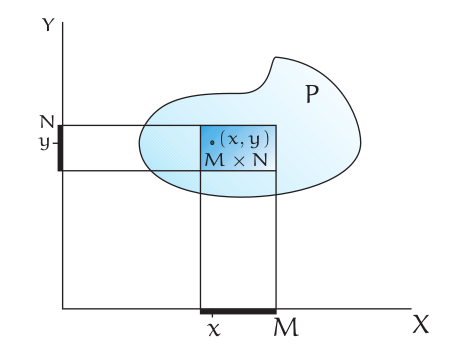
\includegraphics[width=10cm, height=8cm]{images/product_topology.png}
\end{center}

%让$x \in X$,$y \in Y$,我们希望定义一个$(x,y)$的邻域,直觉上邻域里面的点$(x',y')$要尽可能的接近$(x,y)$,那么应该是$x$和$x'$接近,$y$和$y'$接近,这种想法不就是分别去取$x$在$X$和$y$在$Y$里面的邻域吗?但是呢,这样定义出来的$X \times Y$邻域是有问题的,观察上面的图,$M$和$N$分别是$X$和$Y$中$x$和$y$的邻域,按照邻域公理如果一个集合$P$包含$M \times N$,那么$P$也应该是一个邻域,现在你会发现这个形状不规则的$P$,你似乎没办法用$X$和$Y$里面的邻域表示了.

\begin{proof}
先写一下我们的证明思路,要证明上述度量诱导出来的拓扑是乘积拓扑:(1)在乘积拓扑中找邻域,这个邻域在$d$度量诱导的拓扑里面(2)在$d$度量诱导的拓扑里面找邻域,这个邻域在乘积拓扑里面.

(1)在乘积拓扑下,如果一个子集$A \subseteq X \times Y$是$p(p_x,p_y)$邻域,那么存在一个开集含于它,所以我们必须找到这样一个$X \times Y$乘积拓扑里面的开集,乘积拓扑上的开集为$\bigcup(U,V)$,其中$U \in \tau_X$,$V \in \tau_Y$.这样不好操作啊,怎么把前面个bigcup去掉呢?其实可以比较从容的去掉,因为点$p$肯定属于某个$X$开集,开集自包含,同样是$p$的一个邻域.那么我们的命题可以变成下面的样子:

$A$是邻域的充分必要条件是: 分别存在$X$中的开集$U$和$Y$中的开集$V$,使得$p \in U \times V \subseteq A$.如果我们能找到这样的$U$,$V$,进一步我们可以分别找到它们里面分别关于$p_x$的邻域$B_\zeta(p_x)$和$p_y$的邻域$B_\delta(p_y)$。然后我们知道\[B_{min(\zeta,\delta)}(p) \subseteq B_\zeta(p_x) \times B_\delta(p_y)\]其中$B_{min(\zeta,\delta)}(p)$就是一个$d$度量下的邻域,$A$包含它,所以$A$也是$d$度量诱导的拓扑下的邻域.

(2)在$d$度量诱导的拓扑下,任意的$A$邻域包含一个$p=(p_x,p_y)$的一个邻域$B_\varepsilon(p)$,而\[B_\varepsilon(p)=B_\varepsilon(p_x) \times B_\varepsilon(p_y)\],其中$B_\varepsilon(p_x)$和$B_\varepsilon(p_y)$分别是$X$和$Y$下的邻域,各自在找一个开集,所以$A$也是乘积拓扑下的邻域.
\end{proof}


\begin{definition}
对于一个映射$\func{f}{A}{X \times Y}$,设\[f_X = j_X \circ f, \quad f_Y = j_Y \circ f,\]换言之$f(a) \equiv (f_X(a),f_Y(a))$,则称$f_X$,$f_Y$为$f$的分量(component).
\end{definition}

\begin{theorem}
映射$\func{f}{A}{X \times Y}$连续的充分必要条件是两个分量$f_X$和$f_Y$都连续.
\end{theorem}

\begin{proof}
如果$f$连续,由复合映射的连续性可知,$f_X$和$f_Y$也都连续.反过来如果$f_X$和$f_Y$都连续,$f^{-1}(U \times V)=f_X^{-1}(U) \cap f_Y^{-1}(V)$,开集的交还是开集,所以$f$连续.
\end{proof}

\begin{example}
考察平面上的一条参数曲线$x(t)=(x_1(t),x_2(t))$.上面定理告诉我们,$x$连续当且仅当$x_1$,$x_2$都连续.
\end{example}

乘积拓扑?弱拓扑?奇妙...

\newpage
\subsection{Subspace topology}

拓扑空间$X$的一个子集$A$上可以很简单地定义一种非常自然的拓扑结构,称为子空间拓扑.子空间拓扑也是使得含入映射$i \colon A \hookrightarrow X$连续的最弱拓扑.

\begin{definition}
设$(X,\tau)$是个拓扑空间,$A \subseteq X$,令\[\tau|_A=\Set{U \cap A}{U \in \tau}\],则$\tau|_A$是$A$上的一个拓扑,称为$A$上的\textbf{子空间拓扑}(subspace topology),而拓扑空间$(A,\tau|_A)$称为$(X,\tau)$的子空间(subspace).
\end{definition}

\begin{proposition}
设$A$是拓扑空间$(X,\tau)$上的子集,$\func{i}{A}{X}$是一个含入映射,则$A$上由$i$决定的弱拓扑就是子空间拓扑.
\end{proposition}

\begin{proof}
这个命题还是比较显然的,因为$i^{-1}(U)=U \cap A$.
\end{proof}

还有下面几个比较简单的性质:

\begin{proposition}
\begin{enumerate}
	\item 如果$B \subseteq A \subseteq X$,则$\tau|_B = (\tau|_A)|_B.$
	\item $U$是$(A,\tau|_A)$里的开集当且仅当存在$(X,\tau)$中的开集$V$使得$U = V \cap A.$
	\item $U$是$(A,\tau|_A)$里的闭集当且仅当存在$(X,\tau)$中的闭集$V$使得$U = V \cap A.$
\end{enumerate}
\end{proposition}

这里需要非常注意一个东西,无论是开集还是闭集,一定要讲清楚是相对哪个拓扑而言的,这一点非常重要.

\begin{example}
我们来思考一个度量空间上的自然的子空间是什么呢?设$(X,d)$是一个度量空间,度量拓扑为$\tau$.$A$是$X$的子集,则可以在$A$上规定一个自然的度量$d_A$,使得任取$x,y \in A$,$d_A(x,y)=d(x,y)$.任取$a \in A$,考察它在$X$中的一个$\varepsilon$球型邻域$B_\varepsilon=\Set{x \in X}{d(a,x) < \varepsilon}$,你会发现\[B_\varepsilon \cap A = \Set{x \in A}{d(x,y) < \varepsilon}.\]恰好就是$a$在$A$中关于度量$d_A$的$\varepsilon$球形邻域.	
\end{example}


\begin{example}
设$X$和$Y$是两个拓扑空间,$A$是$X$的子空间.此时可以考虑一个映射$\func{f}{X}{Y}$在$A$上的\textbf{限制映射}(restriction map)\[\func{f|_A}{A}{Y},\ x \mapsto f(x).\]
\end{example}

\begin{lemma}
\textbf{粘接引理}(pasting lemma) 设$\{C_1,\ldots,C_n\}$是$X$的一个\textbf{有限覆盖}(finite closed cover),即由有限多个$X$的闭子集构成的子集族,满足$C_1 \cup \ldots \cup C_n=X$.如果映射$\func{f}{X}{Y}$使得每个$f|_{C_k}$都连续,则$f$连续.
\end{lemma}

\begin{proof}
任取$Y$中的闭集$A$,\[\begin{aligned} 
					f^{-1}(A)&=f^{-1}(A) \cap (C_1 \cup \ldots \cup C_n)\\
					&=(f^{-1}(A) \cap C_1) \cup \ldots \cup (f^{-1}(A) \cap C_n).\end{aligned}\]第一行是简单的变换,整理成子空间拓扑形式,因为每个$f|_{C_k}$都连续,所以按照定义${f|_{C_k}}^{-1}(A)=D_K \cap C_k = f^{-1}{A} \cap C_K $在$C_k$中也是闭的,其中$D_k$也是某个闭集,然和有限多个闭集并还是闭集,即$f^{-1}(A)$是闭集.
\end{proof}

\begin{definition}
设$\func{f}{X}{Y}$是连续单射,在$f(X) \subseteq Y$取子空间拓扑,然后考虑映射\[\func{g}{X}{f(X)},\ x \mapsto f(x).\]如果$g$是同胚,则称$f$为\textbf{嵌入}(embedding).
\end{definition}

嵌入是同胚的推广.含入映射就是嵌入的典型例子.


\newpage
\subsection{Quotient map and Quotient space}
和弱拓扑相对应地,有另外一种非常自然的定义拓扑结构的方法叫“强拓扑”,就是利用映射$\func{f}{X}{Y}$把集合$X$上的拓扑结构$\tau$“向右转移”到集合$Y$上去.那么这里为什么叫强拓扑呢?因为使得$f$连续的$Y$上的最小拓扑是平凡拓扑$\{Y,\emptyset\}$.与弱拓扑相反的是取使得$f$连续的$Y$上最强的拓扑(即在对于集合族中是最大的).


\begin{definition}
设有一族拓扑空间$(X_\lambda,\tau_\lambda)$及映射$\func{f_\lambda}{X_\lambda}{Y}$.则$Y$上满足条件使得每个$f_\lambda$都连续的最大拓扑$\tau$称为由这些$f_\lambda$决定的强拓扑(strong topology).
\end{definition}


\end{document}




